
\section{ElasticSearch}

\subsection{Installation}

Die Installation ist bei ElasticSearch dreigeteilt. Um die Suchmaschine in dem Umfang nutzen zu können, wie es hier benötigt wird, muss der komplette ELK-Stack installiert werden. ElasticSearch ist hierbei das Kernstück und dient als Datenbank. Kibana ist eine grafische Benutzeroberfläche und Logstash bildet die Brücke zwischen der Datenquelle und ElasticSearch. Während ElasticSearch Java mitgeliefert hat, muss für Logstash Java Version 8 oder 11 nachinstalliert werden. Um die drei Dienste für den Development Modus zu installieren, müssen nur die Archive entpackt und die entsprechenden Anwendungen gestartet werden. Ohne die Konfigurationsdateien zu ändern, haben die Anwendungen direkt miteinander kommunizieren können. Allerdings hat Logstash ein paar Warnungen beim Start geworfen, welche mit JRuby zusammenhingen und den Entwicklern schon bekannt sind. Daher können diese hier ignoriert werden.

Für eine richtige Installation gibt es mehrere Wege. Für den Test wurde das Debian-Packet verwendet. Alternativ ist es allerdings auch möglich, entweder das Repository von ElasticSearch einzupflegen oder einen Docker-Container zu nutzen. Die Installtion verlief hierbei ohne Probleme.

\subsection{Indexierung}
\label{elaVgl:index}

Um nun Daten zu indexieren, muss in einer Konfigurationsdatei in Logstash definiert werden, wie und welche Daten gelesen und and das ElasticSearch System weitergegeben werden sollen \ref{lst:lsConf}. Dabei kann Logstash direkt MySQL-Abfragen gegen die Datenbank stellen. Die Datei ist in zwei Blöcke unterteilt. Zum einen ein Input-Block, welcher erklärt, welche Daten eingelesen werden sollen und ein Output-Block, welcher das Ziel für die Daten angibt. Für den Input-Block wird der JDBC Treiber von MariaDB verwendet.

Bei diesem Schritt kam es bei dem System allerdings zu Problemen. Der Treiber konnte über den in der Dokumentation angegeben Weg nicht geladen werden. Damit der Treiber korrekt erkannt werden konnte, musste er zusammen mit den Core-Bibliotheken von Logstash geladen werden. Deswegen ist die Zeile mit dem Pfad zur Bibliothek auch leer. 

Nachdem die Datenbank Konfiguration und Abfrage angegeben wurden, kann zudem noch ein Zeitplan definiert werden. Außerdem ist es auch möglich, eine Art Delta-Query zu definieren. Hierfür wird eine Tracking-Spalte festgelegt, welche dann in der Abfrage auf einen Zeitstempel überprüft wird.

Im zweiten Teil der Datei wird das Ziel definiert. Die erste Zeile dient dazu nur dem Debugging, da es alle ausgegeben Linien des Skripts auch auf der Shell ausgibt. 

In dem ElasticSearch-Segment wird zum einen eine ID definiert, welche verhindert, dass Einträge doppelt in die Datenbank gespielt werden. Deswegen wird hier die ID der Lemmata genommen, da diese auch in der Datenbank nicht wiederholt werden darf. Zum Anderen wird noch ein Index angegeben, in welchen die Daten geschrieben werden sollen. 

Als die Indexierung nun gestartet wurde, kam es allerdings zu einem Fehler. Die MySQL-Abfrage sei nicht gültig. Dies lag daran, dass um zu ermitteln, wie viele Daten indiziert werden müssen, die Abfrage mit einer Count-Abfrage umhüllt wird. Dabei verwendete Logstash Double anstelle von Single-Quotes, was bei MariaDB zu einem Fehler führte. Dies konnte behoben werden, indem eine Einstellung in der Datenbank vorgenommen wurde, um auch Double-Quotes zu erlauben. 
Danach verlief die Indexierung ohne weitere Probleme.

\begin{lstlisting}[language=Ruby, frame=single, label={lst:lsConf}] 
input {
  jdbc {
    jdbc_validate_connection => true
    jdbc_driver_library => ""
    jdbc_driver_class => "Java::org.mariadb.jdbc.Driver"
    jdbc_connection_string =>
        "jdbc:mariadb://localhost:3306/dietrichonline"
    jdbc_user => "USER"
    jdbc_password => "PW"
    tracking_column => "timestamp"
    use_column_value=>true
    statement => "MYSQL-Query WHERE timestamp > :sql_last_value"
    schedule => "0 */6 * * *"
  }
}

output {
  stdout { codec => json_lines }
  elasticsearch {
    document_id => "%{id}"
    index => "lemma"
    hosts => "localhost:9200"
  }
}
\end{lstlisting}

Nun ist die Frage jedoch, wie weiß ElasticSearch, was für ein Datentyp das Feld besitzt. Dafür verwendet ElasticSearch ein sogenanntes Dynamic-Mapping, indem es versucht den am besten passenden Datentyp für das Feld zu ermitteln.

Sollen nun bestimmte Feld-Typen verwendet werden, muss der Index von Hand erstellt werden. Um ein Feld zu definieren, muss ein Mapping manuell erstellt werden \ref{lst:mapping}. Dieses enthält zumindest den Feld-Namen und den Typen. Zudem können noch andere Optionen angegeben werden, um die Indexierung nach dem eigenen Ermessen anzupassen. Es kann zum Beispiel deklariert werden, dass ein Feld zwar existiert, allerdings nicht Suchbar ist. Sowas wäre für interne IDs zur Verwaltung interessant,welche nicht nach außen hin herausgegeben werden sollten. Wichtig ist, dass nun nur alle definierten Felder in die Datenbank geschrieben werden. Felder, die aus der Datenbank geladen werden, allerdings nicht im Index vorhanden sind, werden ignoriert.

\begin{lstlisting}[language=JSON, frame=single, label={lst:mapping}] 
PUT lemma
{
  "mappings": {
    "properties": {
      "original_bezeichnung": {
        "type":  "keyword"
}}}}
\end{lstlisting}

Sollen nicht alle Felder von Hand erstellt werden, ist es zudem möglich eine Vorlage für ein dynamisches Feld zu generieren \ref{lst:mappingTemplate}. So kann für ein Feld eine bestimmte Regel gesetzt werden, ohne alle Felder manuell anlegen zu müssen. Als Beispiel habe wurde hier definiert, dass das Feld original\_bezeichnung immer nur als Keyword gespeichert wird.

\begin{lstlisting}[language=JSON, frame=single, label={lst:mappingTemplate}] 
PUT lemma
{
  "mappings": {
    "dynamic_templates": [
      {
        "obez_as_keyword": {
          "match":   "original_bezeichnung",
          "mapping": {
            "type": "keyword"
  }}}]}}
\end{lstlisting}

Für den Test war die Erstellung eines Mappings oder eines dynamischen Templates allerdings nicht notwendig, da ElasticSearch bei der automatischen Indexierung jedes String-Feld als Keyword, sowie Volltext abspeichert, insofern die Länge unter 256 Zeichen ist. So konnte die Abfrage, welche alle Lemmata mit den Buchstaben S sucht einfach verwendet werden, indem das Keyword-Feld zur Suche verwendet wurde.

\subsection{Oberfläche}

Die Oberfläche von Kibana bietet eine zu Beginn überwältigende Erfahrung \ref{img:elasticInterface}. Um dies für spätere Anwender zu verhindern, bietet Kibana die Möglichkeit Sichten für unterschiedliche Nutzer zu erstellen. Zudem kann die Oberfläche hinter ein Login-System geschaltet werden.

Auf der Oberfläche gibt es viele Menüpunkte, welche es ermöglichen die Daten auf diverse Arten darzustellen, darunter in Grafen-Form oder auf einer Landkarte. Unter dem Punkt Management finden sich die Einstellungen für das ElasticSearch System. Hier kann man nicht nur Snapshots erstellen, sondern auch das System mit Updates versorgen. Zudem können hier die Indices verwaltet werden \ref{img:elasticIndexSettings}. Eine Erstellung der Indices ist allerdings nur per API möglich. Es existiert allerdings die Möglichkeit einige Einstellungen an den Indices vorzunehmen und diese auch zu löschen. Zudem gibt es die Möglichkeit Indices eine Lebensdauer zuzuweisen, was in Zeiten der Datenschutzgrundverordnung sicherlich eine nützliche Funktion darstellen wird. 

Die Oberfläche ist vollkommen responsive. Neben diesem Menü gibt es ebenfalls eine Entwicklerkonsole, in der es möglich ist Anfragen an das ElasticSearch-System zu schicken, ohne mit Curl oder ähnlichen zu arbeiten, was das Debugging vereinfacht.

\begin{figure}
	\centering
	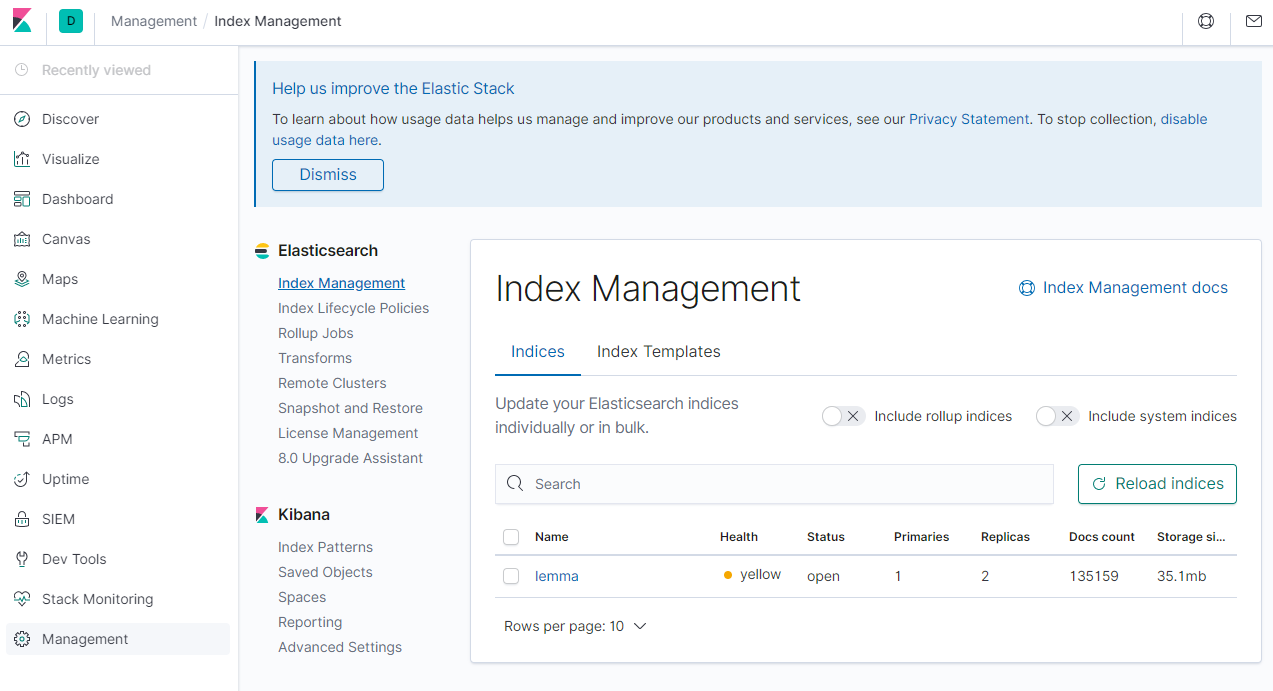
\includegraphics[width=1\linewidth]{images/elastic_ui.png}
	\caption{Index Management Seite von ElasticSearch}
	\label{img:elasticInterface}
\end{figure}


\subsection{Dokumentation}

Die Dokumentation von ElasticSearch ist sehr ausführlich und gut zu lesen. Um einen einfacheren Einstieg in das System zu bieten, beginnt die Dokumentation bei jedem Thema mit einem kleinen Beispiel, um das Konzept zu verdeutlichen. Diese Struktur zieht sich durch die gesamte Dokumentation, jedes Thema ist mit vielen Codeschnipseln bebildert, was eine einfachere Einarbeitung in das System ermöglicht. 
Gut gelöst dabei ist, dass es möglich ist mit einem Klick den Befehl direkt in die Konsole von Kibana zu importieren. Während meines Testes wurde nur ein Fehler in der Dokumentation entdeckt: Bei der Informationsseite zum PHP-Klienten eine falsche PHP-Version vermerkt.

\subsection{Absetzen einer Anfrage und Integration in PHP}

ElasticSearch bietet für PHP einen eigenen Klienten an. Es ist möglich, diesen unter anderem auch mit Composer zu installieren. Um die indexierten Dateien abzufragen, muss ein ClientBuilder gebaut werden, welcher einen oder mehrere Hosts mitgegeben bekommt. Der Server sendet, insofern nicht anders konfiguriert, 10 Resultate zurück. Um diese Limitierung aufzuheben, muss hierbei an 2 Stellen etwas verändert werden. In PHP muss dem Klienten bei der Anfrage ein Parameter mitgegeben werden, welcher die Menge der Ergebnisse bestimmt. Dies funktioniert allerdings nur bis zu 10.000 Ergebnissen. Sollten mehr Ergebnisse erwünscht sein, muss auch noch etwas am Index geändert werden. Dies kann entweder über eine HTTP Anfrage oder über die Oberfläche geändert werden. Für den Test wurde dieses Limit nun erhöht \ref{img:elasticIndexSettings}. 


\begin{lstlisting}[language=php, frame=single, label={lst:phpElastic}, morekeywords={type,uninvertible,indexed,stored,field,multiValued, name}] 
<?php
[...] # Imports and variable declarations

$clientBuilder = ClientBuilder::create()->setHosts(['136.199.34.55']);
$client        = $clientBuilder->build();

$params = [
    'index' => 'lemma',
    'body' => [
        'size' => 1000000,
        'query' => [
            "wildcard" => ["bezeichnung.keyword" => "S*"],
]]];

$results = $client->search($params);
[...] # Loop with Timer  
$results = $client->search($params);

$count=0;
  foreach ($results['hits']['hits'] as $hit){
    $count++;
  }
[...] # Output Runtime
\end{lstlisting}

Zum Code ist noch zu sagen, dass im Ergebnis keine Summe der Ergebnisse liegt, sondern dafür ein eigener Query vonnöten ist. Deswegen werden hier die Ergebnisse in einer Schleife gezählt.

Auch hier wurde nun der Query 100-Mal ausgeführt, um einen Median Wert zu ermitteln. Dieser lag bei ElasticSearch bei 0.58 Sekunden pro Query.

\begin{figure}
	\centering
	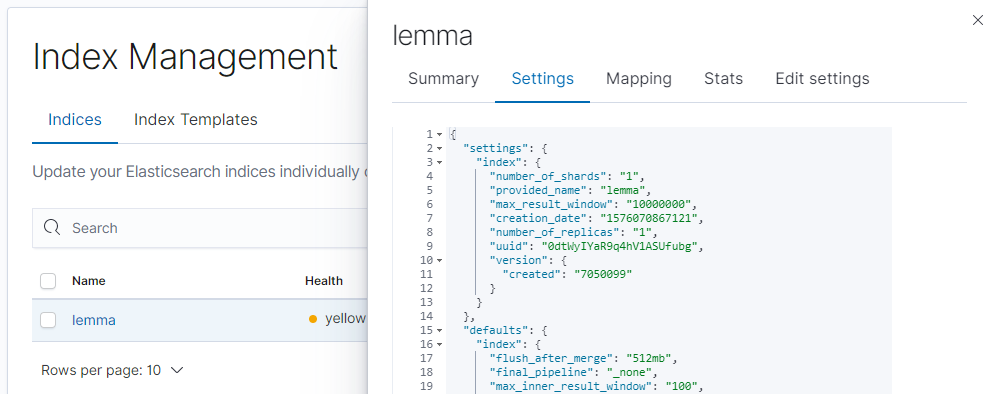
\includegraphics[width=1\linewidth]{images/elastic_index_settings.png}
	\caption{Einstellungen vom Lemma-Index bei ElasticSearch}
	\label{img:elasticIndexSettings}
\end{figure}


